\chapter{Introduction}\label{chap:introduction}

%wofür das alles?
\newcommand{\vehiclecaps}{B}
\newcommand{\vehiclecap}{\beta}
\newcommand{\vehicetype}{v}
\newcommand{\soc}{q}
\newcommand{\places}{\mathcal{X}}
\newcommand{\depot}{\delta}
\newcommand{\depots}{D}
\newcommand{\trips}{\mathcal{T}}
\newcommand{\trip}{\tau}
\newcommand{\chargers}{\mathcal{C}}
\newcommand{\charges}{Z}
\newcommand{\timefunc}{T}
\newcommand{\energyfunc}{Q}
\newcommand{\numbervt}{m}
\newcommand{\chargefunc}{Q^C}
\newcommand{\charge}{\zeta}
\newcommand{\vehicleschedule}{\psi}
\newcommand{\schedule}{\Psi}
\newcommand{\evehicleschedule}{\omega}
\newcommand{\eschedule}{\Omega}
\newcommand{\departure}{d}
\newcommand{\arrival}{a}
\newcommand{\timestart}{s}
\newcommand{\timeend}{e}
\newcommand{\chargestation}{c}
\newcommand{\vehicletypes}{\mathcal{V}}




\section{Motivation}\label{sec:motivation}

Laut \citet{Nie06} ist unser Thema voll wichtig.

\section{Stand der Forschung}

Mehrere Zitate auf einmal: \citet{Nie06,GJ79,KN12}

\chapter{Notation und Grundlegendes}\label{ch:notation}
Die Arbeit sollte so gut wie möglich alle zum Verständnis notwendinge Definition, Notation, Konventionen beinhalten.
Dieser Abschnitt ist dafür geeignet.

\paragraph*{Graphentheorie.} 
Sei~$G=(V,E)$ ein ungerichteter Graph, wobei~$V$ die Knotenmenge und~$E\subseteq \{\{v,w\}\mid v,w\in V,\, v\neq w\}$ die Kantenmenge bezeichnen.
Für einen Graphen~$G$ schreiben wir auch~$V(G)$ und~$E(G)$ für die Knoten- beziehungsweise Kantenmenge von~$G$.

Wenn man viel Notation einzuführen hat, dann kann ein sogenanntes \emph{labeling} empfehlenswert sein.
Wir nennen
\begin{labeling}{$\deg^i_G(v)$}
	\item[$V(G)$] die \emph{Knotenmenge} von~$G$;
	\item[$E(G)$] die \emph{Kantenmenge} von~$G$ mit~$E(G) \subseteq \binom{V(G)}{2}$; die Knoten~$u$ und~$v$ einer Kante~$e = \{u, v\} \in E(G)$ werden \emph{Endpunkte} genannt;
	\item[$n_G$] die Anzahl~$|V(G)|$ der Knoten;
	\item[$m_G$] die Anzahl~$|E(G)|$ der Kanten.
\end{labeling}

\paragraph*{Parametrisierte Komplexität.} 
Wir verwenden Standardnotation aus der Parametrisierten Komplexität und Algorithmik~\cite{Nie06}.

\chapter{\LaTeX{}-Beispiele}

\section{Grundlegendes}
Einzelne Zeilenumbrüche
sind 
Latex egal.
Mit einem doppelten Umbruch

erzeugt man einen neuen Absatz.
Der Übersicht halber sollte man die Zeilen im Latex-Quellcode trotzdem nicht zu lang machen.

Mit newcommand lassen sich eigene Befehle definieren:
\newcommand{\sfe}{supercalifragilisticexpialigetisch}
Jede \sfe{}e Instanz lässt sich mit einem \sfe{}en Algorithmis in \sfe{}er Zeit lösen.
(Sehr nützlich, wenn man später Dinge umbenennen will.)

\section{Formatierung}
\textit{Ich bin kursiv}.
\textbf{Ich bin fett}.
\textsc{Ich bin in Kapitälchen} (für Problemnamen).
\enquote{Ich stehe in Anführungszeichen.}

Hier kommt eine Formel: $a = b + c$.
Die nächste Formel kriegt mehr Platz und wird am \&-Zeichen ausgerichtet:\footnote{Man kann auch an mehreren Stellen ausrichten.}
\begin{align*}
	f : \RR &\to \RR \\
	x &\mapsto x^2
\end{align*}

Ohne Sternchen gibt's Zeilennummern:
\begin{align}
	a &= \abs{x - 2}\\
	b &= \enorm{a + x}\\
	c &= a^2 + b^2 \\
	\sqrt{17} &> 1 \label{eq:wurzel}
\end{align}

Hoch- und tiefgestellt wird so: $x_1, x^2, x_{i,j}^t$

Brüche schreibt man $\frac{n!}{k!(n-k)!}$ oder im Fließtext auch einfach $n!/(k!(n-k)!)$.

Ein paar weitere Operatoren:
\begin{align*}
	\sum_{i=1}^n \int_a^b \lim_{x \to \infty} \max_{y \geq x} \left\{ x \cdot y \middle| \left[ x^2 - y^2 \right] \subseteq \tilde{\Omega} \right\}
\end{align*}

Nützliche Buchstaben: $\ell, \theta, \vartheta, \epsilon, \varepsilon, \phi, \varphi$

Nützliche Relationen: $G \neq H \simeq K \cong T \approx \emptyset$.

Wer den Namen für ein bestimmtes Symbol sucht schaut am besten auf \url{http://detexify.kirelabs.org/}

Wenn man Text innerhalb einer Formel einfügen möchte, muss dieser mit \textit{\textbackslash text} ausgezeichnet werden:
\begin{align*}
	V &= \frac{4}{3} \pi z^3 & \text{Volumen einer Kugel mit Radius $z$}\\
	V &= \pi z^2 a = \pi zza & \text{Volumen einer Pizza mit Radius $z$ und Dicke $a$}
\end{align*}

Versuche Zeilenumbrüche an mathematischen Ausdrücken wie den nun hier folgenden $G$ zu vermeiden. 
Verwende die Tilde im Latex-Code um das zu vermeiden, wie folgt.

Versuche Zeilenumbrüche an mathematischen Ausdrücken wie den nun hier folgenden~$G$ zu vermeiden. 

Und noch was: Sätze sollten auch nicht mit mathematischen Ausdrücken beginnen.
Also, statt \enquote{$G$ ist toll.} besser \enquote{Graph~$G$ ist toll.}.


\section{Theoreme \& Co}


\begin{definition}\label{def:smaller}
	Für $a, b \in \RR$ schreiben wir $a < b$ falls gilt
	\todo[inline]{hier feht noch was. Manchmal ist es sinnvoll etwas lokal statt in \cref{ch:notation} zu definieren.}
\end{definition}

\begin{lemma}[trivial]\label{thm:trivial}
	$a < b \iff b > a$
\end{lemma}
\begin{proof}
	Gilt nach \cref{def:smaller}.
\end{proof}

\begin{theorem}[Robertson, Seymour]
	Die Menge der endlichen Graphen ist wohlquasigeordnet bzgl. der Relation \enquote{$\preceq$}.
\end{theorem}
\begin{proof}
	Folgt aus \cref{thm:trivial} in Verbindung mit \cref{eq:wurzel} (Übungsaufgabe).
\end{proof}

\newcommand{\vertexcover}{\textsc{Vertex Cover}}
\problemdef{\vertexcover{}}
{Ein Graph $G$, $k \in \NN$.}
{$\exists C \subseteq V(G) : \abs{C} = k$ und $\forall e \in E(G): e \cap C \neq \emptyset$?}

\begin{observation}\label{thm:exponentialzeit}
	\textsc{\vertexcover{}} ist lösbar in exponentieller Zeit.
\end{observation}

Aus \cref{thm:exponentialzeit} folgt unmittelbar das folgende \cref{thm:entscheidbar}.

\begin{corollary}\label{thm:entscheidbar}
	\textsc{\vertexcover{}} ist entscheidbar.
\end{corollary}

\begin{example}
	Ein interessantes Beispiel.
\end{example}

\begin{remark}
	Eine Anmerkung.
\end{remark}


\section{Abbildungen}

Beispiele für Graphen sind in \cref{fig:graph} abgebildet.
Hierbei ist \cref{fig:directed_graph} ein \textit{gerichteter Graph} (auch \textit{Digraph}).

Wer zu faul ist, die Bilder in tikz zu erstellen, kann sich auch \url{http://ipe.otfried.org/} anschauen.

\begin{figure}[t]
	\centering
	\tikzstyle{alter}=[circle, minimum size=16pt, draw, inner sep=1pt] 
	\tikzstyle{majarr}=[draw=black]
	\begin{subfigure}[t]{.45\textwidth}
		\centering
		\begin{tikzpicture}[auto, >=stealth',shorten <=1pt, shorten >=1pt]
			\node[alter] at (0,0) (a) {$a$};
			\node[alter, right = 8ex of a] (b) {$b$};
			\node[alter, right = 8ex of b] (c) {$c$};
			
			\draw[majarr] (a) edge (b);
			\draw[majarr] (b) edge (c);
			\draw[majarr] (a)[bend left=43] edge (c);
		\end{tikzpicture}
		\caption{ungerichtet}
		\label{fig:undirected_graph}
	\end{subfigure}  
	\begin{subfigure}[t]{.45\textwidth}
		\centering
		\begin{tikzpicture}[auto, >=stealth']
			\tikzstyle{majarr}=[draw=black,->,shorten <=1.5pt, shorten >=1.5pt]
			\node[alter] at (0,0) (a) {$a$};
			\node[alter, right = 8ex of a] (b) {$b$};
			\node[alter, right = 8ex of b] (c) {$c$};
			
			\draw[majarr] (a) edge node[midway, anchor=south] {$\scriptstyle 1$} (b);
			\draw[majarr] (b) edge node[midway, anchor=south] {$\scriptstyle 2$} (c);
			\draw[majarr] (a) edge[bend left=43] node[midway, anchor=south] {$\scriptstyle 3$} (c);
		\end{tikzpicture}
		\caption{gerichtet}
		\label{fig:directed_graph}
	\end{subfigure}
	\caption{Beispiele für Graphen. Achtung: \textit{label} immer \textbf{nach} \textit{caption}, sonst gehen die Verweise kaputt.}
	\label{fig:graph}
\end{figure}



\Cref{tab:some-table} ist eine große Tabelle.
Normalerweise versucht Latex selbst, einen geeigneten Ort für Abbildungen zu finden.

Externe Bilder lassen sich auch einbinden (siehe \cref{fig:comic}).

\begin{table}[t]
	\caption{\normalfont
		Ergebnisse der Laufzeitexperimente. Alle Zeiten sind in Sekunden angegeben.
		Im Gegensatz zu Abbildungen, Tabellenüberschriften sind über der Tabelle zu platzieren.
	}
	\centering
	\footnotesize
	\renewcommand{\tabcolsep}{7pt}
	\begin{tabular}{ll rr rrr}
		\toprule
		&	file 				& $n$ 		& $m$  		& \texttt{WCC} [s]&\texttt{HKN} [s]	& \texttt{CHLS} [s] \\
		\midrule
		\multirow{4}{*}{\rotatebox[origin=c]{90}{Clustering}} 
		& email 				& 1K	 	& 5K	 	& 0.67 		& 48.75 		& 2.51 	 \\
		& hep-th 				& 7K	 	& 15K	 	& 0.43 		& 1.35 			& 3.75 	 \\
		& netscience 			& 1K	 	& 2K	 	& 0.24 		& 0.37 			& 0.07 	 \\
		& PGPgiantcompo 		& 10K	 	& 24K	 	& 0.67 		& 1.70 			& 3.51 	 \\
		\midrule
		\multirow{4}{*}{\rotatebox[origin=c]{90}{Co-author}} 
		& citationCiteseer 		& 268K	 	& 1.1M		& 21.46 	& 83.90 		& --- 	 \\
		& coAuthorsCiteseer 	& 227K	 	& 0.8M	 	& 11.46 	& 50.35 		& --- 	 \\
		& coAuthorsDBLP 		& 289K	 	& 0.9M		& 15.76 	& 78.51 		& --- 	 \\
		& coPapersCiteseer 		& 434K	 	& 16M		& ---		& ---			& --- 	 \\
		\bottomrule
	\end{tabular}
	\label{tab:some-table}
\end{table}

\begin{figure}
	\centering
	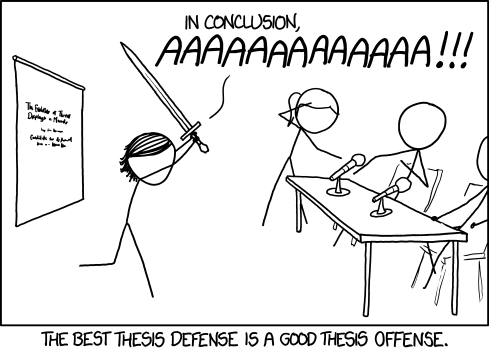
\includegraphics[scale=0.7]{figures/thesis_defense.png}
	\caption{MY RESULTS ARE A SIGNIFICANT IMPROVEMENT ON THE STATE OF THE AAAAAAAAAAAART \cite{xkcd1403}}
	\label{fig:comic}
\end{figure}


\pgfplotstableread[col sep = comma]{example-data.csv}\data % read the csv-file
\begin{table}
	\small
	\caption{\normalfont Bonustabelle (automatisch generiert aus example-data.csv) Die Beschriftung ist immer über Tabellen aber unter Bildern...}
	\pgfplotstabletypeset[columns={graphname,vertices,edges, mmtime,kerneltime,kernelvertices,kerneledges,kmmtime},
	columns/graphname/.style={string type,column name=Graph,column type = {r}},
	columns/vertices/.style={column name=$n$,precision=1,column type = {r}},
	columns/edges/.style={column name=$m$,precision=1,column type = {r}},
	columns/mmtime/.style={column name=blossom5,fixed,precision=2,dec sep align,preproc/expr={0.001*##1 + 0.01}},
	columns/kerneltime/.style={column name=kernel,fixed,precision=2,dec sep align,preproc/expr={0.001*##1 + 0.01}},
	columns/kernelvertices/.style={column name=$n'$,precision=1,column type = {r}},
	columns/kerneledges/.style={column name=$m'$,precision=1,column type = {r}},
	columns/kmmtime/.style={column name=blossom5',precision=2,fixed,dec sep align,preproc/expr={0.001*##1 + 0.01}},
	every head row/.style ={before row=\toprule, after row=\midrule},
	every last row/.style ={after row=\bottomrule}]{\data}
\end{table}


\section{Pseudocode}

\Cref{alg:euclid} ist Euklids Algorithmus zur Bestimmung des größten gemeinsamen Teilers zweier Zahlen.
Die Schleife in \cref{line:loop} terminiert sobald $a$ durch $b$ teilbar ist.

Für mehr Informationen zu Pseudocode in \LaTeX, empfiehlt sich ein Blick in die algorithmicx-Anleitung \cite{algorithmicx}.



\begin{algorithm}
	\caption{Euklids Algorithmus}\label{alg:euclid}
	\begin{algorithmic}[1]
		\Input{$a, b \in \NN$}
		\Output{Der größte gemeinsame Teiler von $a, b$}
		\Function{Euklid}{$a,b$}
		\State $r\gets a\bmod b$ \Comment{$r$ ist der Rest der Ganzzahl-Division $a / b$}
		\While{$r\not=0$} \label{line:loop}
		\State $a\gets b$
		\State $b\gets r$
		\State $r\gets a\bmod b$
		\EndWhile
		\State \textbf{return} $b$
		\EndFunction
	\end{algorithmic}
\end{algorithm}


\chapter{Conclusion}

Ein Fazit is keine Zusammenfassung.
Grob sollten hier erzielte Ergebnisse diskutiert und ein Ausblick für weitere Forschung gegeben werden.

Wir habe dieses tolle Ergebnis.
Allerdings blieb diese andere tolle Frage offen.
Wir vermuten, dass die Frage positive zu beantworten ist wegen diesem tollen Argument.